\documentclass[addpoints]{exam}
\usepackage{cmbright}
\usepackage{amsmath}
\usepackage{amssymb}
\usepackage{graphicx}
\usepackage{multicol}
\usepackage{url}
\usepackage{mhchem}
\setlength\fillinlinelength{2em}

\header{CHE 525: math for CBEE's}{homework \#7}{fall 2025}

\begin{document}

\begin{multicols}{2}
	a manometer is a U-shaped tube with both ends open and a liquid trapped inside. 

	suppose the right side of the tube is always exposed to the atmosphere.
	as for the left side, it was exposed to a pressurized gas line for $t<0$. but, at $t=0$, the line to the high-pressure gas was disconnected. thus, the left side is exposed to the atmosphere as well for $t\geq 0$. 
	consequently, the liquid in the tube at $t=0$ initializes (a) at rest and (b) with a taller height (by $h_0$ m) on the right side.

our goal is to model the difference in the liquid level between the two sides of the tube $h=h(t)$ [m] (by definition, $h>0$ implies the liquid level is lower on the left side).

\columnbreak

        \begin{centering}
            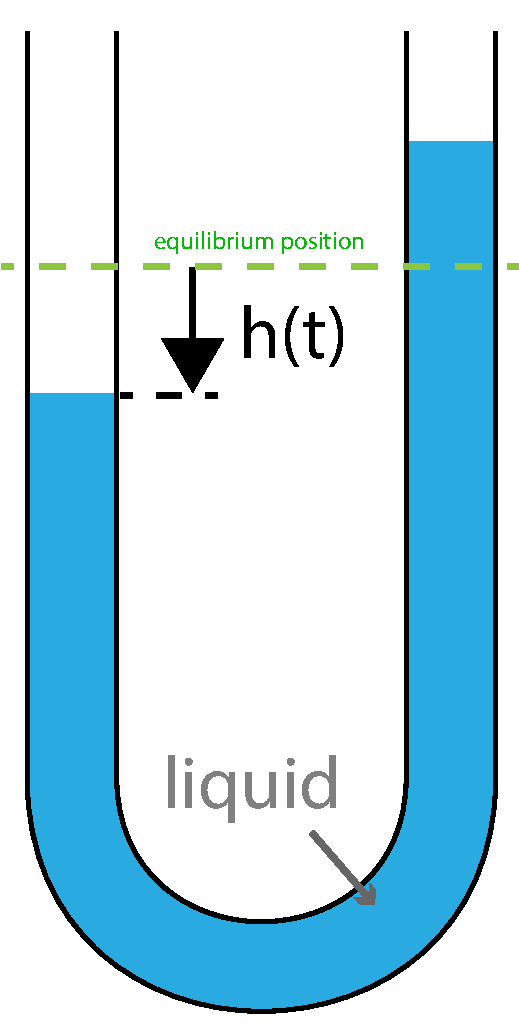
\includegraphics[width=0.1\textwidth]{manometer.pdf}
        \end{centering}

\end{multicols}

\begin{questions}

        
\question derive a dynamic model for $h=h(t)$ [m] for $t\geq 0$ by writing a force balance on the liquid (mass $\times$ acceleration = sum of forces), accounting for (i) the gravitational force and (ii) the viscous forces internal to the liquid.
    the [constant] parameters are listed in the table below.
    consider
    \begin{itemize}
        \item the mass of liquid in the tube is $\rho \pi R^2 L$ [kg].
        \item the restoring force from gravity, due to displaced liquid, is $\pi R^2 \rho g h(t) $ [N].
        \item the viscous force, according to the Hagen-Poiseuille equation, is $8\pi \mu L \frac{dh}{dt}$ [N].
    \end{itemize}

        
%            \begin{equation*}
%        \rho R^2 L \frac{d^2h}{dt^2} = - R^2 \rho g h(t) - 8 \mu L \frac{dh}{dt} 
%        % \frac{d^2h}{dt^2} + \frac{6\mu}{R^2\rho}\frac{dh}{dt} + \frac{3}{2}\frac{g}{L}h(t) = \frac{3}{4\rho L}p(t), 
%        \label{eq:h}
%    \end{equation*} 
          





        % check unit consistency
        % all units: m/s^2
        % dh/dt term:
        %  = m / s * Pa s / m^2 /kg * m^3
        %  = [N/m^2]  m^2 /kg 
        %  = [kg⋅m/s2/m^2]  m^2 /kg 
        %  = m/s2
        % h term:
        %  m/s^2 yeah.
        % forcing term:
        %   = N / m2 / (kg/m^3) / m
        %   = N / (kg)
        %   = m/s2
        \begin{center}
        \begin{tabular}{ c c }
         parameter & description  \\
         \hline
         \multicolumn{2}{c}{\textbf{manometer setup}} \\
         $R$ & radius of the tube [m] \\ 
         $L$ & total length of liquid in tube [m]\\
         \multicolumn{2}{c}{\textbf{properties of the liquid}} \\
         $\rho$ & density [kg/m$^3$]\\
         $\mu$ & viscosity [N$\cdot$s/m$^2$] \\
         \multicolumn{2}{c}{\textbf{a physical constant}} \\
         $g$ & standard acceleration due to gravity [m/s$^2$]
        \end{tabular}
    \end{center}

\question write the second-order ODE you obtain for $h(t)$ as a system of first-order differential equations in matrix-vector form:
\begin{equation*}
	\frac{d \mathbf{x}(t)}{dt}=A\mathbf{x}(t).
\end{equation*}

\question suppose the manometer tube (on earth, $g=9.8\,m/s$^2$) has $R=0.01$\,m and $L=0.2$\,m; olive oil ($\rho=997$\,kg/m$^3$, $\mu=0.001$ Pa$\cdot$s) inside; and begins with $h_0=0.05$\,m. compute the eigenvalues and eigenvectors of the coefficient matrix $A$ in Julia (they should be complex). based on these eigenvalues and eigenvectors, write the solution to $\mathbf{x}(t)$ in the time domain. plot $h(t)$ in Julia.

 
\end{questions}
\end{document}
